\documentclass[12pt]{article}
\pagestyle{empty}
\usepackage{amsmath, amssymb, amsthm}
\usepackage{latexsym, epsfig, ulem, cancel, multicol, hyperref}
\usepackage{graphicx, tikz, subfigure,pgfplots}
\usepackage[margin=1in]{geometry}
\setlength{\parindent}{0pt}
\usepackage{multirow}
\usepackage{mathtools}


\usepackage{verbatim}
\usepackage{tikz}
\usepackage{pgfplots}


\newcommand{\T}[0]{\top}
\newcommand{\F}[0]{\bot}
\newcommand{\liminfty}[1]{\lim_{#1 \to \infty}}
\newcommand{\limzero}[1]{\lim_{#1 \to 0}}
\newcommand{\Z}{\mathbb{Z}}
\newcommand{\R}{\mathbb{R}}
\newcommand{\C}{\mathbb{C}}
\newcommand{\Q}{\mathbb{Q}}
\newcommand{\odd}[0]{\mathbb{Z} - 2\mathbb{Z}}
\newcommand{\lineint}[1]{\int_{#1}}
\newcommand{\pypx}[2]{\frac{\partial #1}{\partial #2}}
\newcommand{\divg}{\nabla \cdot}
\newcommand{\curl}{\nabla \times}
\newcommand{\dydx}[2]{\frac{d #1}{d #2}}
\newcommand{\sqbkt}[1]{\left[ #1 \right]}
\newcommand{\paren}[1]{\left( #1 \right)}
\newcommand{\tribkt}[1]{\left< #1 \right>}
\newcommand{\abso}[1]{\left|#1 \right|}
\newcommand{\zero}{\{0\}}
\newcommand{\then}{\rightarrow}
\newcommand{\nonneg}{\Z^+ \cup \{0\}}
\DeclarePairedDelimiter\ceil{\lceil}{\rceil}
\DeclarePairedDelimiter\floor{\lfloor}{\rfloor}
\newcommand{\union}[2]{\bigcup_{#1}^{#2}}
\newcommand{\inter}[2]{\bigcap_{#1}^{#2}}
\newcommand{\openclose}[1]{\left( #1 \right]}
\newcommand{\closeopen}[1]{\left[ #1 \right)}

\newcommand{\defcomp}{\exists r,s\in \Z^+ \paren{n=rs \wedge \paren{1<r<n} \wedge \paren{1<s<n}}}
\newcommand{\defprime}{\forall r,s \in \Z ^+ \paren{n=rs \rightarrow \paren{r = 1 \wedge s = n}\veebar \paren{r=n \wedge s=1}}}

\newcommand{\wsnumber}{1}
\newcommand{\wstopic}{Vectors}
\pgfplotsset{
    every linear axis/.append style={
       axis x line=center,
       axis y line=center,
       xlabel={$x$},
       ylabel={$y$}
    },
    every axis plot/.append style={thick,mark=none}
}
\tikzset{
    point/.style={circle,draw,fill,minimum width=0.3ex,inner sep=0pt,outer sep=0pt},
    every label/.append style={black}
}


\usepackage[margin=1in]{geometry}
\usepackage{amsmath, amssymb, amsthm, graphicx, hyperref}
\usepackage{enumerate}
\usepackage{fancyhdr}
\usepackage{multirow, multicol}
\usepackage{tikz}
\pagestyle{fancy}
\fancyhead[RO]{Dennis Li}
\fancyhead[LO]{Summer 6W2 2024 MA-UY 2314}
\usepackage{comment}
\newif\ifshow
\showfalse

\ifshow
  \newenvironment{solution}{\textbf{Solution.}}{}
\else
  \excludecomment{solution}
\fi

\renewcommand{\thefootnote}{\fnsymbol{footnote}}
\usepackage{comment}


\newtheorem*{remark}{Remark}


\begin{document}

\begin{center}
\ifshow
  \textbf{\Large Homework 4 Solution}\\
\else
  \textbf{\Large Homework 4}\\
\fi
Due: Tuesday July 30\\via Gradescope\\
\end{center}

\hrule

\vspace{0.2cm}

\begin{enumerate}[$\bullet$]  
\item Late homework is not accepted.  Lateness due to technical issues will not be excused.  
\end{enumerate}

\hrule

\vspace{0.5cm}



\begin{enumerate}
    \item Use mathematical induction to prove
    \[
    \sum_{a=1}^{b}\sum_{c=1}^{d} (a+c) = \frac{bd(b+d+2)}{2} \;\; \forall (b,d) \in \Z^+ \times \Z^+
    \]
    \begin{proof}
        Base Case: let $d=1$
        \[
        \sum_{a=1}^{b}\sum_{c=1}^{1} (a+c) = \frac{bd(b+d+2)}{2}
        \]
        this becomes
        \[
        \sum_{a=1}^{b}\sum_{c=1}^{1} (a+c) = \frac{b(b+3)}{2}
        \]
        Inductive Case: let $k \in \Z^+ : k \geq 1$, and if we let $d=k$, we have
        \[
        \sum_{a=1}^{b}\sum_{c=1}^{k} (a+c) = \frac{bk(b+k+2)}{2}
        \]
        Examine term for $k+1$
        \[
        \sum_{a=1}^{b}\sum_{c=1}^{k+1}(a+c)
        =\sum_{a=1}^{b}\sqbkt{\sum_{c=1}^{k+1}(a+c)}
        \]
        We expand the sum
        \[
        \sum_{a=1}^{b}\sqbkt{\sum_{c=1}^{k}(a+c) + (a+k+1)}
        = \sum_{a=1}^{b}\sum_{c=1}^{k}(a+c) + \sum_{a=1}^{b}(a+k+1)
        \]
        We see that the first half is simply 
        \[
        \sum_{a=1}^{b}\sum_{c=1}^{k}(a+c) = \frac{bk(b+k+2)}{2}
        \]
        Now we work on the second half
        \[
        \sum_{a=1}^{b}(a+k+1) = \sum_{a=1}^{b} a + \sum_{a=1}^{b} (k+1)
        \]
        by definition, we have
        \[
        \sum_{a=1}^{b} a = \frac{b(b+1)}{2} \quad \sum_{a=1}^{b} (k+1) = b(k+1)
        \]
        put everything together, we have 
        \[
        \sum_{a=1}^{b}\sum_{c=1}^{k+1}(a+c) = \frac{bk(b+k+2)}{2} + \frac{b(b+1)}{2} + b(k+1)
        \]
        \[
        = \frac{bk(b+k+2)}{2} + \frac{b(b+1)}{2}  + \frac{2b(k+1)}{2}
        \]
        put the fraction together, we have
        \[
        = \frac{b^2k+bk^2+4bk+b^2+3b}{2}
        \]
        factor it, we have
        \[
        \sum_{a=1}^{b}\sum_{c=1}^{k+1}(a+c)=
        \frac{b(k+1)(b+k+1+2)}{2}
        \]
        
    
        
    \end{proof}
    
    \newpage
    
    \item Section 5.2 \#14,18
        \begin{enumerate}
            \item[14.] Show that for all integer $n \geq 0$
            \[
            \sum_{i=1}{n+1} i \cdot 2^i = n \cdot 2^{n+2} + 2
            \]
            \begin{proof}
            Examine base case when $n=0$:
            \begin{align*}
            &\sum_{i=1}{0+1} i \cdot 2^i = 0 \cdot 2\\
            &= 0 \cdot 2 ^{0+2} + 2
            \end{align*}
            Inductive Step: let $k \in \Z : k \geq 0$, then we have
            \[
            \sum_{i=1}{k+1} i \cdot 2^i = k2^{k+2}+2
            \]
            Assume $k+1$, we have
            \[
            \sum_{i=1}{k+2} i \cdot 2^i = 
            \sum_{i=1}{k+1} i \cdot 2^i + 
            \]
            With induction hypothesis, we have
            \[
            =(k+1)2^{k+2} +  k2^{k+2}+2
            \]
            expand the parenthesis, we have
            \[
            =k2^{k+2}+2^{k+2} + k2^{k+2}+2
            \]
            factoring out $2^{k+2}$, we have
            \[
            =2^{k+2}\paren{2k+2}+2
            \]
            factoring out a $2$, and by algebra, we have
            \[
            =2^{(k+1)+2}(k+1)+2
            \]
            
            \end{proof}

            \item[18.] Show that for all integer $n\geq 2$
                \[
                \prod_{i=2}^{n} \paren{1 - \frac{1}{i}} = \frac{1}{n}
                \]
            \begin{proof}
                Base Case: $n=2$
                \begin{align*}
                    &\prod_{i=2}^{2} \paren{1 + \frac{1}{i}}\\
                    &= 1 - \frac{1}{2}\\
                    &= \frac{1}{2}
                \end{align*}
                Inductive Step: let $ k \in \Z : k \geq 2$, we have
                \[
                \prod_{i=2}^{k} \paren{1 + \frac{1}{i}} = \frac{1}{k}
                \]
                Suppose $k+1$, then
                \[
                \prod_{i=2}^{k+1} \paren{1 - \frac{1}{i}} = \sqbkt{\prod_{i=2}^{k} \paren{1 + \frac{1}{i}}} \cdot \paren{1 - \frac{1}{k+1}}
                \]
                by induction hypothesis, we have
                \[
                = \frac{1}{k}\paren{1 - \frac{1}{k+1}}
                \]
                by algebra, we have
                \[
                =\frac{1}{k} - \frac{1}{k+1} =  \frac{k + 1 -1}{k(k+1)}
                \]
                and finally
                \[
                \prod_{i=2}^{k+1} \paren{1 - \frac{1}{i}} = \frac{1}{k+1}
                \]
                    
            \end{proof}
            

            
        \end{enumerate}

    \item Section 5.2 \#40. let $\mathbb{P}$ denotes the set of all prime numbers, Show that
        \[
        \forall p \in \mathbb{P} \paren{p \geq 5 \then p \left| \sum_{i=1}^{p}i^2\right.}
        \]
        \begin{proof}
            let $n \in \Z$ and $p \in \mathbb{P}: p \geq 5$, we can form the following sum
            \[
            \sum_{i=n}^{n+(p-1)}i^2 = n^2 + (n+1)^2 +\cdots +\paren{n+\paren{p-1}}^2
            \]
            \[
             \sum_{i=n}^{n+(p-1)}i^2 = \sum_{i=0}^{p-1} \paren{i+n}^2
            \]
            notice that
            \[
            \sum_{i=1}^{p} \paren{i+n}^2 = \sum_{i=0}^{p-1} \paren{i+n}^2 
            \]
            we can keep working on the expression
            \[
            =\sum_{i=0}^{p-1} \paren{n^2 + 2ni+i^2} = \sum_{i=0}^{p-1} n^2 + 2n\sum_{i=0}^{p-1} i + \sum_{i=0}^{p-1}i^2
            \]
            \[
            = pn^2 + 2n\paren{\frac{p(p-1)}{2}} + \frac{p(p-1)(2p-1)}{6}
            \]
            and we can factor $p$ and get
            \[
            =p\paren{n^2 + 2n\paren{\frac{(p-1)}{2}} + \frac{(p-1)(2p-1)}{6}}
            \]
            since $p \in \odd$, let $p = 2k+1$ for some $k \in \Z$, we see that
            \[
            \frac{p-1}{2} = \frac{2k+1-1}{2} = k
            \]
            which means this fraction produces an integer. similarly, the term $\frac{(p-1)(2p-1)}{6}$ is also an integer since integer is closed under addition and multiplication. And the entire sum can be written as
            \[
            \sum_{i=1}^{p} \paren{i+n}^2 = p\paren{n^2 + 2n\paren{\frac{(p-1)}{2}} + \frac{(p-1)(2p-1)}{6}}
            \]
            where $\paren{n^2 + 2n\paren{\frac{(p-1)}{2}} + \frac{(p-1)(2p-1)}{6}}$ is an integer since integer is closed under addition and multiplication. therefore we may conclude that
            \[
            p \left| \sum_{i=1}^{p}i^2\right.
            \]
        \end{proof}
    
    
    \newpage
    \item Section 5.3 \#3, 12, 21
        \begin{enumerate}
            \item[3.] Stamps are sold in packages containing either 5 stamps or 8 stamps.
                \begin{enumerate}[a.] 
                    \item Show that $\{5, 8,10,13,15,16,20,21,24,25\}$ can be written as a linear combination of $5$ and $8$
                        \begin{align*}
                            5 = 5\times 1 + 8 \times 0\\
                            8 = 5 \times 0 + 8 \times 1\\
                            10 = 5 \times 2 + 8 \times 0\\
                            13 = 5 \times 1 + 8 \times 1\\
                            15 = 5 \times 3 + 8 \times 0\\
                            16 = 5 \times 0 + 8 \times 2\\
                            20 = 5 \times 4 + 8 \times 0\\
                            21 = 5 \times 1 + 8 \times 2\\
                            24 = 5 \times 0 + 3 \times 8\\
                            25 = 5 \times 5 + 8 \times 0
                        \end{align*}

                    \item Show that any integer of at least 28 can be written as a linear combination of $5$ and $8$.
                        \begin{proof}
                            Basis step:
                            \[
                            28 = 5\times 4 + 8 \times 1
                            \]
                            Inductive step: let $k \in \Z : k \geq 28$. Suppose 
                            \[
                            \exists x,y \in \Z^+ \cup \zero
                            \paren{k = 5x+8y}
                            \]
                            since $k \geq 28$, $y > 2 \vee y \leq 2$, suppose $y \leq 2$, then $x\geq 3$. Define 
                            \[
                            a \coloneqq x-3 \in \Z^+ \cup \zero \quad b\coloneqq y +2 \in \Z^+ \cup \zero
                            \]
                            we now have 
                            \[
                            5a + 8b = 5x-15 + 8y+16 = 5x+8y +1
                            \]
                            notice that $k = 5x+8y$, and we obtained $5a+8b = k+1$ via induction hypothesis. Now we turn to the second case. Suppose $y > 2$, since $y \in \Z$, then $y \geq 3$. Since $k \geq 28$, define the follows
                            \[
                            b \coloneqq y-3 \in \Z^+ \cup \zero \quad a \coloneqq x+5 \in \Z^+ \cup \zero
                            \]
                            we now have
                            \[
                            5a+8b = 5x+25+8b-24 = 5x+8b +1
                            \]
                            notice that $k = 5x+8y$, and we obtained $5a+8b = k+1$, via induction hypothesis.

                        \end{proof}

                        \item[12.] Show that
                            \[
                            \forall n \in \nonneg \paren{5 \mid \paren{7^n - 2^n}}
                            \]
                            \begin{proof}
                                Base Case: n = 0
                                \[
                                7^0 - 2^0 = 0 = \frac{0}{5} 
                                \]
                                Inductive Step: let $k \in \Z : k \geq 0$, and by quotient remainder theorem, for some $q \in \Z$
                                \[
                                7^k - 2^k =5q
                                \]
                                we have
                                \[
                                7^k = 5q + 2^k
                                \]
                                Now examine $k+1$
                                \[
                                7^{k+1}-2^{k-1}
                                \]
                                by algebra 
                                \[
                                7\cdot 7^k - 2\cdot 2^k 
                                \]
                                and by substitution and induction hypothesis
                                \begin{align*}
                                    7\paren{5q + 2^k} - 2\cdot 2^k \\
                                    35q + 7\cdot 2^k - 2\cdot 2^k \\
                                    2^k\paren{7-2}+35q \\
                                    5\cdot 2^k + 35q \\
                                    5\paren{2^k + 7q} 
                                \end{align*}
                                We see that $2^k + 7q$ is integer since integer is closed under multiplication and addition. and let $2^k + 7q = q' \in \Z$, we can rewrite the expression as follows
                                \[
                                7^{k+1} - 2^{k+1} = 5q'
                                \]
                                
                            \end{proof}

                        \item[21.] Prove that
                            \[
                            \sqrt{n} < \sum_{m=1}^{n} \frac{1}{\sqrt{m}}
                            \]
                            for some $n \in \Z : n \geq 2$
                            \begin{proof}
                                Basis step:
                                \[
                                1 < 2
                                \]
                                \[
                                1< \sqrt{2}
                                \]
                                \[
                                2 < \sqrt{2} + 1
                                \]
                                \[
                                \sqrt{2} < \frac{1}{1} + \frac{1}{\sqrt{2}}
                                \]
                                Inductive Step: let $k \in \Z$ and $k \geq 2$. Suppose 
                                \[
                                \sqrt{k} < \sum_{m=1}^{k}\frac{1}{\sqrt{m}}
                                \]
                                Now we make the observation that
                                \begin{align*}
                                    &0<2\leq k\\
                                    &k^2 < k^2+k = k(k+1)\\
                                    &k < \sqrt{k}\sqrt{k+1}\\
                                    &k+1 < \sqrt{k}\sqrt{k+1}+1\\
                                    &\frac{k+1}{\sqrt{k+1}} < \sqrt{k} + \frac{1}{k+1}\\
                                    & \textcolor{red}{\sqrt{k} < \sum_{m=1}^{k}\frac{1}{\sqrt{m}}}\\
                                    & \textcolor{blue}{\sqrt{k+1}} < \textcolor{red}{ \sqrt{k} } + \frac{1}{\sqrt{k+1}} \\
                                    &= \textcolor{blue}{\sum_{m=1}^{k+1}\frac{1}{\sqrt{m}}}
                                    & \text{via Induction Hypothesis}\\ 
                                \end{align*}

                            \end{proof}
                        
                \end{enumerate}

        \end{enumerate}

    \newpage

    \item Section 5.3 \#27,28
        \begin{enumerate}
            \item[27.] A sequence $d_1,d_2,\ldots$ is defined by letting $d_1=2$ and $d_k = \frac{d_{k-1}}{k}$ for each integer $k \geq 2 $. Show that for every integer $n\geq 1$, $d_n = \frac{2}{n!}$.
                \begin{proof}
                    Base case: 
                    \[
                    d_1 = 2 = \frac{2}{1} = \frac{2}{1!}
                    \]
                    Inductive step: let $m \in \Z : m \geq 1$. We have
                    \[
                    d_m = \frac{2}{m!}
                    \]
                    examine $d_{m+1}$, we have
                    \[
                    d_{m+1} = \frac{d_m}{m+1}
                    \]
                    Substitute via induction hypothesis
                    \[
                    d_{m+1} = \frac{2}{m!} \cdot \frac{1}{m+1} = \frac{2}{\paren{m+1}!}
                    \]

                \end{proof}
            \item[28.] Prove that for every integer $n \geq 1$,
                \[
                \frac{1}{3} = \frac{1+3+5 + \cdots + \paren{2n-1}}{\paren{2n+1}+\paren{2n+3}+\cdots + \paren{2n + \paren{2n-1}}}
                \]
                \begin{proof}
                    Suppose an integer $k \geq 1$
                        \[
                        \frac{\sum_{i=1}^{k}2i-1}{ \sum_{i=1}^{k}2k +2i-1} 
                        \]
                    distribute the sum, we have
                        \[
                        \frac{2\cdot \sum_{i=1}^{k}i - \cdot \sum_{i=1}^{k}1 }{2k^2 + 2 \cdot \sum_{i=1}^{k} - \cdot \sum_{i=1}^{k}1}
                        \]
                    carry out the individual sum, we have
                        \[
                        \frac{k\paren{k+1}-k}{2k^2 + k\paren{k+1}-k}
                        \]
                    simplify into
                        \[
                        \frac{k^2+k-k}{2k^2 + k^2 + k -k} = \frac{k^2}{3k^2} = \frac{1}{3}
                        \]
 
                \end{proof}
                
        \end{enumerate}
        \newpage
        \item Section 5.3 \#33, 45, 46
            \item[33.] Consider a $4 \times 6$ checkerboard. Draw a covering of the board by $L $ shaped trominoes.

            \begin{figure}[!h]
                \centering
                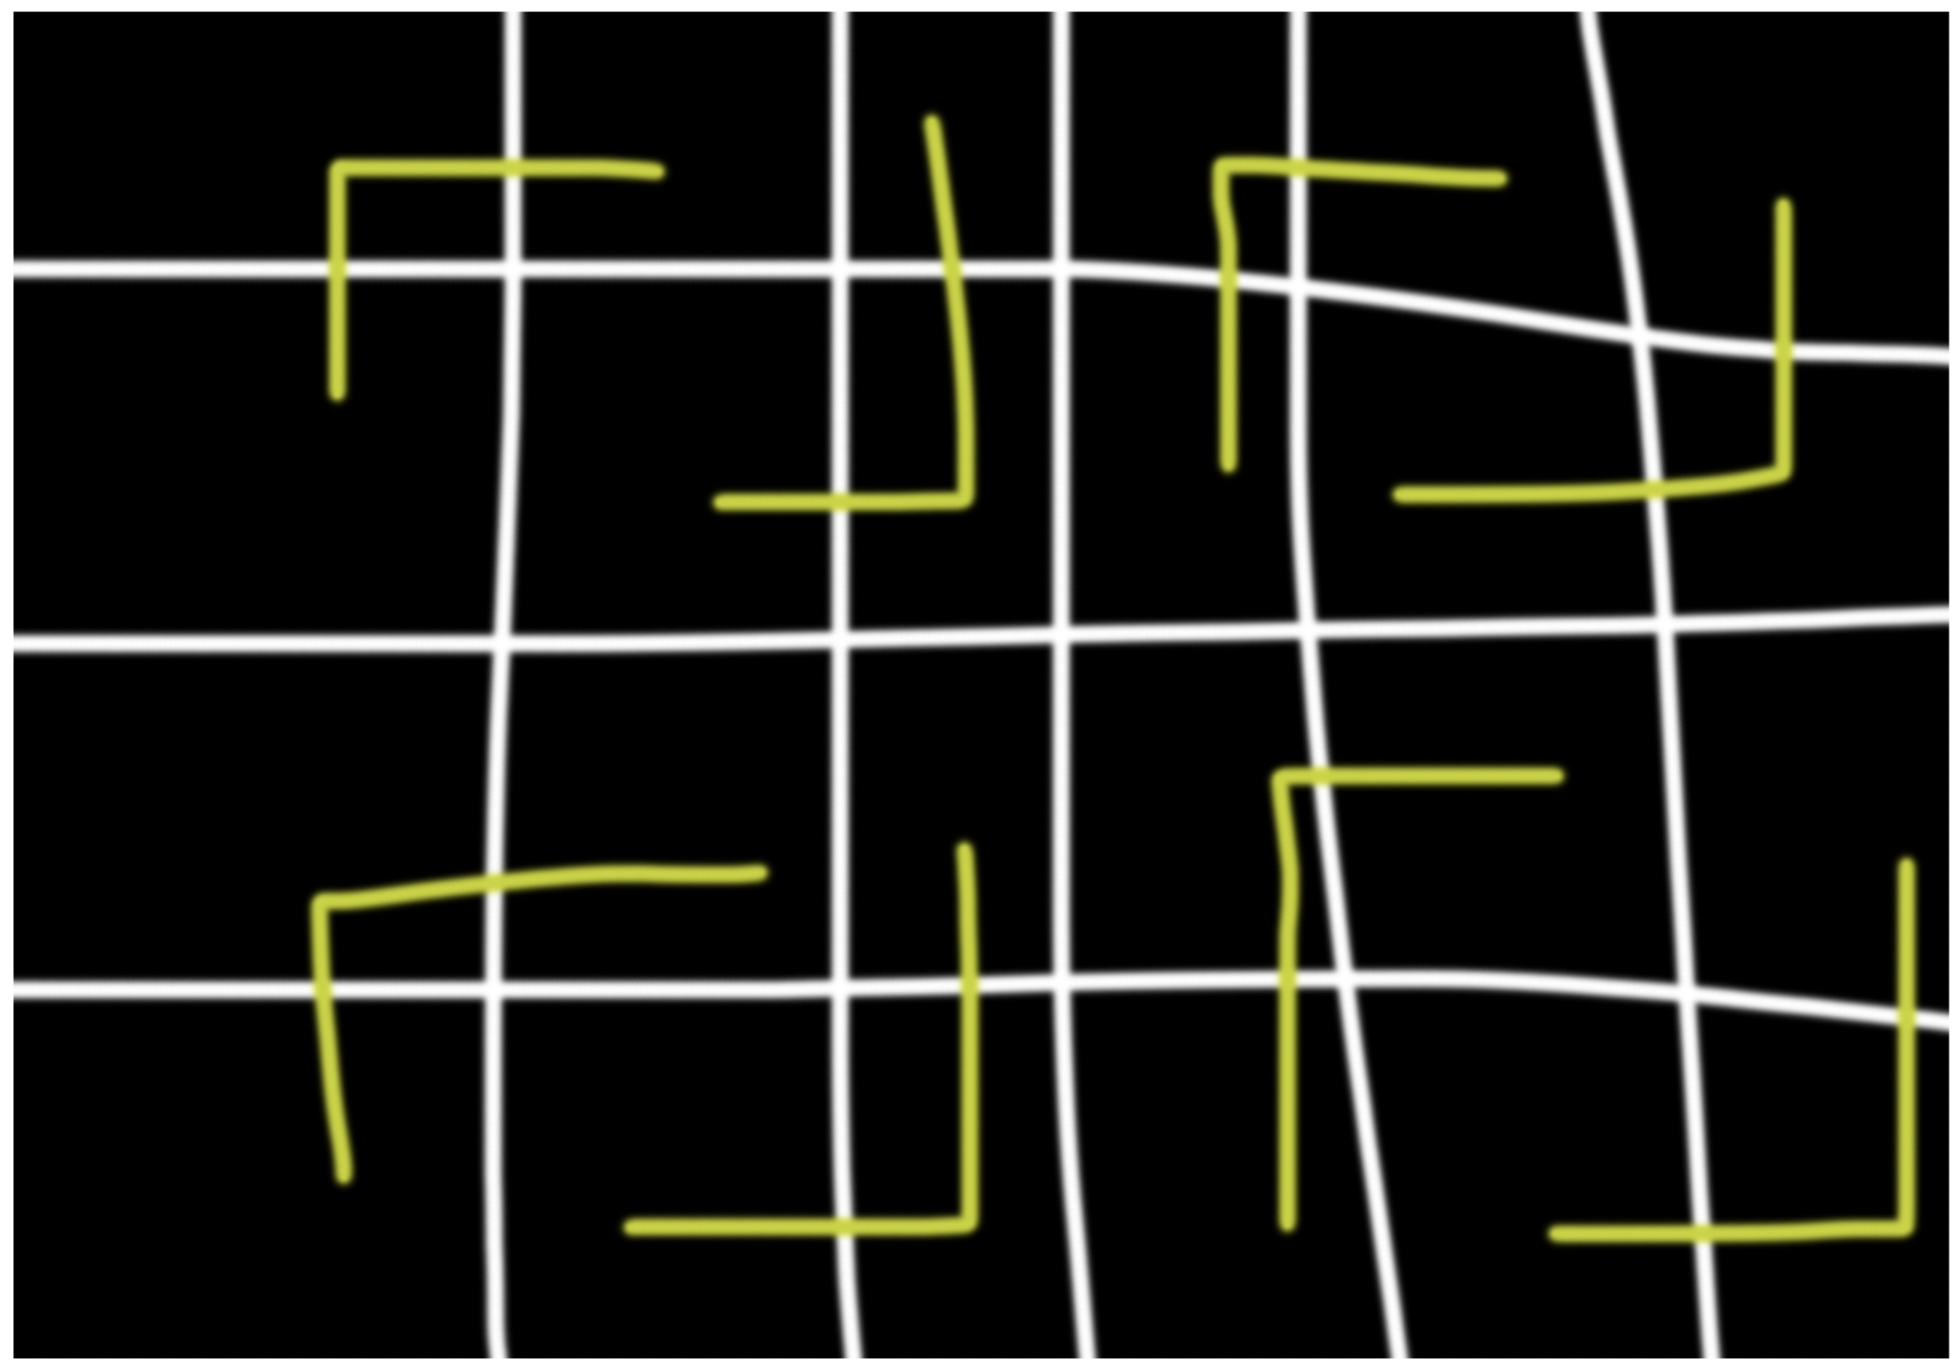
\includegraphics[width=0.25\linewidth]{Picture Folder//HW02/HW04_5.3-33.png}
                \caption{Weird Picture for 5.3-33}
                \label{fig:5.3-33}
            \end{figure}

            \item[45.] The inductive step failed to go from $n=1$ to $n=2$, and $k=1$, which invalidate the proof, since there is no set C that be defined with the given definition. When $k=1$, there are only 2 elements in set $A$ and one element in set $B$, meaning that no $2^{nd}$ element can be removed from set $B$ to define the set $C$, hence the inductive step is erroneous. 

            \item[46.] The basis step is not true, since $3^1-2=1$ is odd, therefore not even, hence the inductive step following it is erroneous. 

        \newpage

        \item Section 5.3 \#36. Show that there can be a team that beats any other team in a round robin game with $n\geq 2$ teams of participants.
            \begin{proof}
                Base case: when $n=2$, let $T, T'$ be 2 distinct teams. There are two cases
                \[
                \begin{cases}
                    T \text{ beats } T'\\
                    T'\text{ beats } T
                \end{cases}
                \]
                since there are no ties, we can label them with $T_1$ and $T_2$. Now for the inductive step, let $k \geq 2$, and the teams can be put labeled as 
                \[
                \mathbf{A} = \{T_{1},T_{2},\ldots,T_{k-1},T_k \}
                \]
                such that $T_i$ beats every team for $i = 1,2,\ldots,k-1$. Now examine $k+1$. To do so we introduce a new team $T'$, and investigate 3 cases.
                    \begin{enumerate}[I.]
                        \item $T'$ wins every team, we can therefore define the sequence as follows
                            \[
                            T'=T_1 \quad T_1 = T_2 \cdots \textit{ etc.}
                            \]
                            All previous index of the team are moved one element forward, we have obtained a new sequence in the form
                            \[
                            \mathbf{A'} = \{T_1, T_2, \ldots, T_k, T_{k+1} \}
                            \]
                            This shows that it is possible to label it in such way if $T'$ beats every team.
                        \item $T'$ Looses to every team, in this case we set the following
                            \[
                            T' = T_{k+1}
                            \]
                            And we obtain the following
                            \[
                            \mathbf{A'} = \{T_1, T_2, \ldots, T_k, T_{k+1} \}
                            \]
                            This shows that it is possible to label it in such way if $T'$ loses to every team.
                        \item $T'$ wins $m$ amount of teams for some integer $1 \leq m < k$, we can define $T' = T_{m+1}$ and the the sequence is demonstrated as follows
                            \[
                            \mathbf{A'} = \{T_1, T_2, \ldots, T_{m},T_{m+1},\ldots,T_{k+1} \}
                            \]
                            with the introduction of another team, we added 1 to $k$. This showed that it is possible to label it in such way if $T'$ beats $m$ teams.
                    \end{enumerate}
               
                
            \end{proof}
    \newpage
    \item Section 5.4 \#13, 20
        \begin{enumerate}
            \item[13.] Any integer greater than 1 is divisible by a prime number or is a prime number.
                \[
                \forall n \in \Z \; \exists p \in \mathbb{P} \paren{
                n > 1 \then p \mid n
                }
                \]
                \begin{proof}
                    Basis step: $2 \mid 2$ since $2 = 2\times 1$ for some $1 \in \Z$, and $2 \in \mathbb{P}$.\\
                
                    Inductive step: let $k \in \Z$ and $k \geq 2$. Suppose there exists a prime $p > 1$ such that $p \mid i$ for all $i \in \{ 2,\ldots,k\}$. We see that $k$ is either prime of composite. \\
                    \textbf{Case prime:} suppose $k+1 \in \mathbb{P}$, we see that
                    \[
                    (k+1) \mid (k+1)
                    \]
                    since $ k+1 = (k+1) \times 1$ for some $1 \in \Z$ and $k+1 \in \mathbb{P}$. Now we look at the other case.\\
                    \textbf{Case composite:} Suppose $k+1$ is not a prime, or $k+1$ is composite.
                    \[
                    \defcomp
                    \]
                    therefore $k+1 = rs$ and $1<r<k+1$ and $1<s<k+1$ for some $r,s\in\Z^+$. Since everything is integer, we have $2 \leq r \leq k$ and $2 \leq s \leq k$. So there exists a prime $p>1$ such that $p \mid r$ via strong induction hypothesis. Also since
                    \[
                    r \mid (k+1) \then p \mid (k+1)
                    \]
                    via transitivity of divides. Therefore any integer greater than $1$ is either prime or have prime factors, or, is a prime.
                
                \end{proof}

            \item[20.] Suppose that $b_1,b_2,b_3,\ldots,$ is a sequence defined as
                \[
                b_1 = 0, \quad b_2 = 3, \quad b_k=5\cdot b_{\floor{k/2}} + 6
                \]
                for all integer $k \geq 3$. Prove that $b_n$ is divisible by 3 for each integer $n \geq 1$
                \begin{proof}
                    Base case: suppose $n=1$ and $n=2$, we have the following
                        \[
                        b_1 = 0, \quad 3 \mid 0
                        \]
                        \[
                        b_2 = 3, \quad 3 \mid 3
                        \]
                    Inductive step: suppose that for all integer $m \geq 2$ such that for all integer $i$ and $1 \leq i \leq m$, $3 \mid b_i$. By the definition of the sequence, we have the following
                        \[
                        b_{m}=5\cdot b_{\floor{m/2}} + 6
                        \]
                    We would break it into 2 cases to examine $m+1$. \\
                    \textbf{Case 1 Even:}First we assume $m+1 \in 2\Z$, we have $m = 2n_1$ for some $n_1 \in \Z$. The expression of the term would be
                        \[
                        b_{m+1}=5 \cdot b_{\floor{\paren{2n_1}/2}} + 6
                        \]
                    which simplifies to
                        \[
                        b_{m+1}=5 \cdot b_{\floor{\paren{n_1}}} + 6
                        \]
                    Since
                        \[
                        \floor{n_1} = n_1
                        \]
                    therefore
                        \[
                        b_{m+1}=5 \cdot b_{\paren{n_1}} + 6
                        \]
                    since $m = 2n_1$ and $m \geq 3$, we have
                        \[
                        m+1 \geq \frac{m+1}{2} = n_1 \geq 1
                        \]
                    Therefore by strong induction hypothesis, $b_{n_1}$ is divisible by 3, we can rewrite it as $b_{n_1} = 3q_1$ for some $q_1 \in \Z$, and obtain
                        \[
                        b_{m+1}=5 \cdot \paren{3q_1} + 6
                        \]
                    we can factor a 3 out and obtain   
                        \[
                        b_{m+1} = 3\cdot \paren{5q_1 + 2}
                        \]
                    we see that $5q_1 +2$ is an integer since integer is closed under multiplication and addition, therefore $3 \mid b_{m+1}$\\
                    \textbf{Case 2 Odd:}Here we assume $k+1 \in \odd$, we have $m = 2n_2+1$ for some $n_2 \in \Z$. The expression of the term would be 
                        \[
                        b_{m+1}=5 \cdot b_{\floor{\paren{2n_2+1}/2}} + 6
                        \]
                    which simplifies to
                        \[
                        b_{m+1}=5 \cdot b_{\floor{\paren{n_2+1/2}}} + 6
                        \]
                    since
                        \[
                        \floor{\frac{2n_2+1}{2}} = \floor{n_2 + \frac{1}{2}} = n_2
                        \]
                    therefore
                        \[
                        b_{m+1}=5 \cdot b_{n_2} + 6
                        \]
                    since $m+1 = 2n_2+1$, we have $m = 2_{n_2}$ and
                        \[
                        m \geq \frac{m}{2} = n_2 \geq 1
                        \]
                    Therefore by strong induction hypothesis, $b_{n_2}$ is divisible by 3, we can rewrite it as $b_{n_2} = 3q_2$ for some $q_2 \in \Z$, and obtain
                        \[
                        b_{m+1}=5 \cdot \paren{3q_2} + 6
                        \]
                    we can factor a 3 out and obtain   
                        \[
                        b_{m+1} = 3\cdot \paren{5q_2 + 2}
                        \]
                    we see that $5q_2 +2$ is an integer since integer is closed under multiplication and addition, therefore $3 \mid b_{m+1}$
                    And we have proven in both cases that $3 \mid b_{m+1}$.
                    
                \end{proof}
        \end{enumerate}

    \item Consider the Fibonacci sequence $f_0 = f_1 = 1$ and $f_m = f_{m-1} + f_{m-2}$ for all $m \geq 2$. Use Strong mathematical induction to prove that, for any integer $n \geq 0$, 
        \[
        f_n = \frac{1}{\sqrt{5}}\sqbkt{\paren{\frac{1+\sqrt{5}}{2}}^{n+1} - \paren{\frac{1-\sqrt{5}}{2}}^{n+1}}
        \]
        \begin{proof}
            Consider the base case $n=0$, we have the following
                \[
                f_0=\frac{1}{\sqrt{5}}\sqbkt{\paren{\frac{1+\sqrt{5}}{2}}^{0+1} - \paren{\frac{1-\sqrt{5}}{2}}^{0+1}} 
                \]
                \[
                = \frac{1}{\sqrt{5}}\paren{\frac{1+\sqrt{5}-1+\sqrt{5}}{2}} = \frac{1}{\sqrt{5}}\cdot\frac{2\sqrt{5}}{2} = 1
                \]
            Now consider $n=1$, we have
                \[
                f_1=\frac{1}{\sqrt{5}}\sqbkt{\paren{\frac{1+\sqrt{5}}{2}}^{1+1} - \paren{\frac{1-\sqrt{5}}{2}}^{1+1}} 
                \]
                \[
                =\frac{1}{\sqrt{5}} \paren{
                \frac{1 + 2\sqrt{5} + 5 }{4}-
                \frac{1 - 2\sqrt{5} + 5 }{4}
                }=\frac{1}{\sqrt{5}}\frac{4\sqrt{5}}{5} = 1
                \]
            Inductive step: suppose for all integer $k \geq 1$, for all $i \in \Z : 0 < i \leq k$, the following stands
                \[
                f_k = \frac{1}{\sqrt{5}}\sqbkt{\paren{\frac{1+\sqrt{5}}{2}}^{k+1} - \paren{\frac{1-\sqrt{5}}{2}}^{k+1}}
                \]
            since the element $f_k$ is defined as
                \[
                f_k = f_{k-1}+ f_{k-2}
                \]
            and $k \geq 2$.\\
            now we have $k+1$ in the form by definition of Fibonacci sequence
                \[
                f_{k+1} = f_{k}+f_{k-1}
                \]
            Since $k \in \{0,1,\ldots,k \}$ and $k-1 \in \{0,1,\ldots,k \}$, by strong induction hypothesis,
                \[
                f_k = \frac{1}{\sqrt{5}}\sqbkt{\paren{\frac{1+\sqrt{5}}{2}}^{k+1} - \paren{\frac{1-\sqrt{5}}{2}}^{k+1}}
                \]
            and
                \[
                f_{k-1} = \frac{1}{\sqrt{5}}\sqbkt{\paren{\frac{1+\sqrt{5}}{2}}^{k} - \paren{\frac{1-\sqrt{5}}{2}}^{k}}
                \]
            if we write $f_{k+1}$ in terms of their sum
                \[
                f_{k+1} = \frac{1}{\sqrt{5}}\sqbkt{\paren{\frac{1+\sqrt{5}}{2}}^{k+1} - \paren{\frac{1-\sqrt{5}}{2}}^{k+1}}
                +
                \frac{1}{\sqrt{5}}\sqbkt{\paren{\frac{1+\sqrt{5}}{2}}^{k} - \paren{\frac{1-\sqrt{5}}{2}}^{k}} 
                \]
            factoring to get
                \[
                f_{k+1} = \frac{1}{\sqrt{5}} \sqbkt{\paren{\frac{1+\sqrt{5}}{2}}^{k+1} - \paren{\frac{1-\sqrt{5}}{2}}^{k+1} + 
                \paren{\frac{1+\sqrt{5}}{2}}^{k} - \paren{\frac{1-\sqrt{5}}{2}}^{k}}
                \]
            keep factoring to get
                \[
                f_{k+1} = \frac{1}{\sqrt{5}}\sqbkt{
                \paren{\frac{1+\sqrt{5}}{2}}^{k}\paren{\frac{1+\sqrt{5}}{2} + 1}
                -
                \paren{\frac{1-\sqrt{5}}{2}}^{k}\paren{\frac{1-\sqrt{5}}{2} +1}
                }   
                \]
            simplifying, we have
                \[
                f_{k+1} = \frac{1}{\sqrt{5}}\sqbkt{
                \paren{\frac{1+\sqrt{5}}{2}}^{k}\paren{\frac{3+\sqrt{5}}{2}}
                -
                \paren{\frac{1-\sqrt{5}}{2}}^{k}\paren{\frac{3-\sqrt{5}}{2}}
                }
                \]
            we multiply the numerator and the denominator by 2 for the following terms
                \[
                f_{k+1} = \frac{1}{\sqrt{5}}\sqbkt{
                \paren{\frac{1+\sqrt{5}}{2}}^{k}\paren{\frac{6+2\sqrt{5}}{4}}
                -
                \paren{\frac{1-\sqrt{5}}{2}}^{k}\paren{\frac{6-2\sqrt{5}}{4}}
                }
                \]
            We notice that, this is
                \[
                f_{k+1} = \frac{1}{\sqrt{5}}\sqbkt{
                \paren{\frac{1+\sqrt{5}}{2}}^{k}\paren{\frac{1+\sqrt{5}}{2}}^2
                -
                \paren{\frac{1-\sqrt{5}}{2}}^{k}\paren{\frac{1-\sqrt{5}}{2}}^2
                }
                \]
            which is 
                \[
                f_{k+1}=\frac{1}{\sqrt{5}}\sqbkt{\paren{\frac{1+\sqrt{5}}{2}}^{k+2} - \paren{\frac{1-\sqrt{5}}{2}}^{k+2}}
                \]
                
                
            
        \end{proof}

    \newpage
    \item Section 5.4 \#25, 32
        \begin{enumerate}
            \item[25.] The proof stated that the hypothesis holds between $0 \leq i \leq k$. However, the induction was applied erroneous since the writer as not established the behavior of $r^{k-1}$, which is not defined by the writer. 
            \item[32.] The induction hypothesis states that to prove this universally qualified statement, one have to show $P(k)\equiv \T$ and $P(k+1)\equiv \T$. However, the writer used $P(3k)$ instead, which is outside the definition of mathematical induction. By the provided definition, we see that $P(0),P(1),P(2),P(3),P(6)$ is true, without having information of anything else, therefore we cannot build a sound argument on top of this as it cant \textit{propagate} itself for the universally qualified statement. A counter example being 
            \[
            P(n)\coloneqq 0 \leq n \leq 2 \vee 3 \mid n
            \]
            We see that this statement is true for $P(0),P(1),P(2),P(3),P(6)$, but not for $P(4),P(5)$
            
        \end{enumerate}
    \newpage
    \item Suppose you wish to show that $P(n)$ is true for all integers $n \geq a$. You begin by defining the set
        \[
        S =  \{ n \geq a : n \in \Z \wedge P(n) \equiv \F\}
        \]
        Your goal is to show that $S = \varnothing$
        \begin{enumerate}[a.]
            \item Explain why $S$ has a smallest element in your contradiction proof.
            \item[Ans:] If the set $S$ is not empty, that means the following. First, the set is bounded below by $a$ since $n \geq a$. Secondly, this is a set of integers. Thirdly, we assumed the set to not be empty. Therefore, by the \textbf{Well-Ordering Principle}, the set has to contain a smallest element.
            \\
            \item If you know that $P(a)$ is $\T$, then explain why the smallest element of $S$, denoted by $x$, satisfies $x>a$ in your contradiction proof.
            \item[Ans.] If we know that $P(a)$ is true, then it is not part of the set $S$. And as since the set has a smallest element by the well-ordering principle, there exist some $a$ such that $P(a) = \bot$. Since the set is bounded below by $a$ and $a$ is not part of the set, then $x\neq a \wedge x > a$.
            \\
            \item Explain why $P(x)$ is $\T$ and $P(x-1)$ is $T$ in your contradiction proof.
            \item[Ans.] If $P(x)$ is $\bot$, and it is the smallest element in the set, we know that $P(x-1)$ has to be $\top$ since it not being $\T$ contradicts with $x$ being the smallest element in the set since $x-1 < x$.
            \\
            \item Suppose you do not know that $P(a)$ is $T$, explain why you cannot say $P(x-1)$ is $T$ in your contradiction proof. 
            \item[Ans.] If $P(a)=\top$ is not given, then we cannot make the assertion that $a \notin S$, therefore we cannot comment on if $x$ is the smallest element in the set, because it could very well be $a$, which in turn invalidate the statement above claiming $P(x-1) = \top$ 
        \end{enumerate}

        \newpage

    \item Section \#5.4 26,27
        \begin{enumerate}
            \item[26.] Use the well-ordering principle for the integers to prove that: Every integer greater than 1 is divisible by a prime number.
            \begin{proof}[proof 5.4.26]
                Let $S$ be a set defined as follows:
                \[
                S = \{ n \in \Z^+ - \{1\} : \text{$n$ is not divisible by a prime number}\}
                \]
                We see that the set has is bounded below by $1$, and the set is composed of integers. Assume that $S \neq \varnothing$, the set satisfies the well-ordering principle. This means that the set contains a smallest element, which will be denoted as $l$. We examine 2 cases:\\
                \textbf{Case 1:} Suppose $l$ is prime, then it has a prime factor which is $l$ itself, which contradicts with the definition of the set $S.$\\
                \textbf{Case 2:} Suppose $l$ is composite, then by the definition of composite numbers, we can write it as $l = rs$ for some $r,s \in \Z^+$ such that $1 < r < l$ and $1 < s < l$. Since $r,s < l$, we know that $r,s \notin S$, since $l$ is the smallest element in the set. However, $r,s \notin S$ implies that for some $p \in \mathbb{P}$, $p \mid r$ and $p \mid s$, and by transitivity of divides, $p \mid l$, which contradicts with the definition of the set. We can therefore conclude that the assumption $S \neq \varnothing$ leads to a contradiction, therefore we accept 
                \[
                S = \varnothing
                \]
                and this in turn proves the original statement. 
            \end{proof}

            \item[27.] Use the well-ordering principle for the integers to prove the existence part of the unique factorization of integers theorem, in other words, prove that every integer greater than 1 is either prime or a product of prime numbers. 
                \begin{proof}[proof 5.4.27]
                    let $S$ be a set defined as below
                    \[
                    S = \{ n \in \Z^+ - \{1\} : \text{$n$ is not prime and not a product of prime numbers}\}
                    \]
                    We see that the set has is bounded below by $1$, and the set is composed of integers. Assume that $S \neq \varnothing$, the set satisfies the well-ordering principle. This means that the set contains a smallest element, which will be denoted as $l$. We examine 2 cases:\\
                    \textbf{Case 1:} Suppose $l$ is prime, then it contradicts with the definition of the set, which means $l \notin S$.\\
                    \textbf{Case 2:} Suppose $l$ is composite, then by the definition of composite numbers, we can write it as $l = rs$ for some $r,s \in \Z^+$ such that $1 < r < l$ and $1 < s < l$. Since $r,s < l$, we know that $r,s \notin S$, since $l$ is the smallest element in the set. However, $r,s \notin S$ implies that $r,s$ must be either prime or products of prime numbers. Thus $l$ itself can be written as a product of these primes, contradicting the assumption that $l\in S$. Both cases lead to a contradiction based on the assumption that $S \neq \varnothing$, we conclude 
                    \[
                    S = \varnothing
                    \]
                    and this in turn proves the original statement. 
                \end{proof}
            
        \end{enumerate}
    \newpage

    \item Section 6.1 \#6, 15(b)(c), 18
        \begin{enumerate}
            \item[6.] Define the following sets for some integer $a,b,c$ 
                \[
                A = \{ x \in \Z : x = 5a + 2 \}
                \]
                \[
                B = \{ y \in \Z : y= 10b - 3 \}
                \]
                \[
                C = \{ z \in \Z : z= 10c + 7 \}
                \]
                Prove or disprove 
                    \begin{enumerate}[a.]
                        \item $A \subseteq B$
                            \begin{proof}[disproof]
                                Choose $a = 0 \in \Z$, we have the element $x = 2$. We see that
                                \[
                                2 = 10b - 3
                                \]
                                \[
                                5 = 10b
                                \]
                                \[
                                b=\frac{1}{2} \notin \Z
                                \]
                                We have found $x \in A \wedge x \notin B$, which disproof the statement. 
                            \end{proof}
                        \item $B \subseteq A$
                            \begin{proof}
                                Assume an arbitrarily chosen integer $y \in B$, assume $y \in A$, we have the following relationship
                                \[
                                10b-3 = 5a+2
                                \]
                                for some integer $b$ and $a.$ now we do some algebra to get
                                \[
                                10b -5 = 5a
                                \]
                                \[
                                2b - 1 = a
                                \]
                                we see that $2b-1$ and $a$ are both integers since integer is closed under multiplication and subtraction, we see that every element in $B$ can be expressed as an element in $A$, which means $y \in A \wedge y \in B$ for any arbitrary $y$, therefore 
                                \[
                                B \in A
                                \]
                                
                            \end{proof}
                        \item $B = C$
                            \begin{proof}
                                Assume an arbitrarily chosen integer $z\in C$, it can be written as $z = 10c + 7$ for some integer $c$. Assume $z \in B$, we have the following
                                \[
                                10c+7 = 10b-3
                                \]
                                through algebra, we get
                                \[
                                10c = 10b-10
                                \]
                                and 
                                \[
                                c = b-1
                                \]
                                which also means 
                                \[
                                b=c+1
                                \]
                                We see that $z =10(c+1)-3 $ and $y = 10(b-1)+7$ and $10$ This means that for any arbitrarily chosen element in $C$, it can be written in terms of an element in $B$, and vice versa. Therefore $B \subseteq C \wedge C \subseteq B$ and this means $B=C$
                            \end{proof}
                    \end{enumerate}

                \item[15.] In each of the following, draw a venn diagram for sets A,B,C that satisfy the given condition.
                    \begin{enumerate}
                        \item[b.] $A \subseteq B$, $C \subseteq B$, $A \cap C \neq \varnothing$
                        \begin{figure}[!h]
                            \centering
                            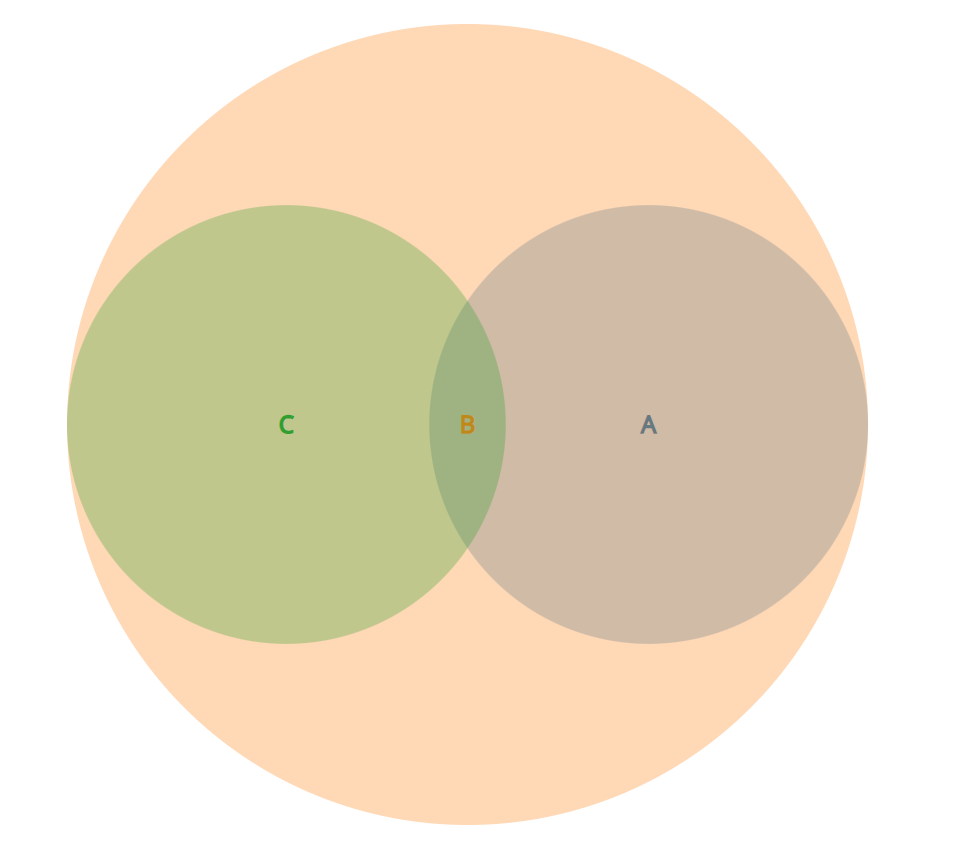
\includegraphics[width=0.3\linewidth]{Picture Folder//HW02/6-1-15-b.png}
                            \caption{6.1.15-b}
                            \label{fig:6.1.15-b}
                        \end{figure}

                        \item[c.] $A \cap B \neq \emptyset, \ B \cap C \neq \emptyset, \ A \cap C = \emptyset, \ A \nsubseteq B, \ C \nsubseteq B$
                        \begin{figure}[!h]
                            \centering
                            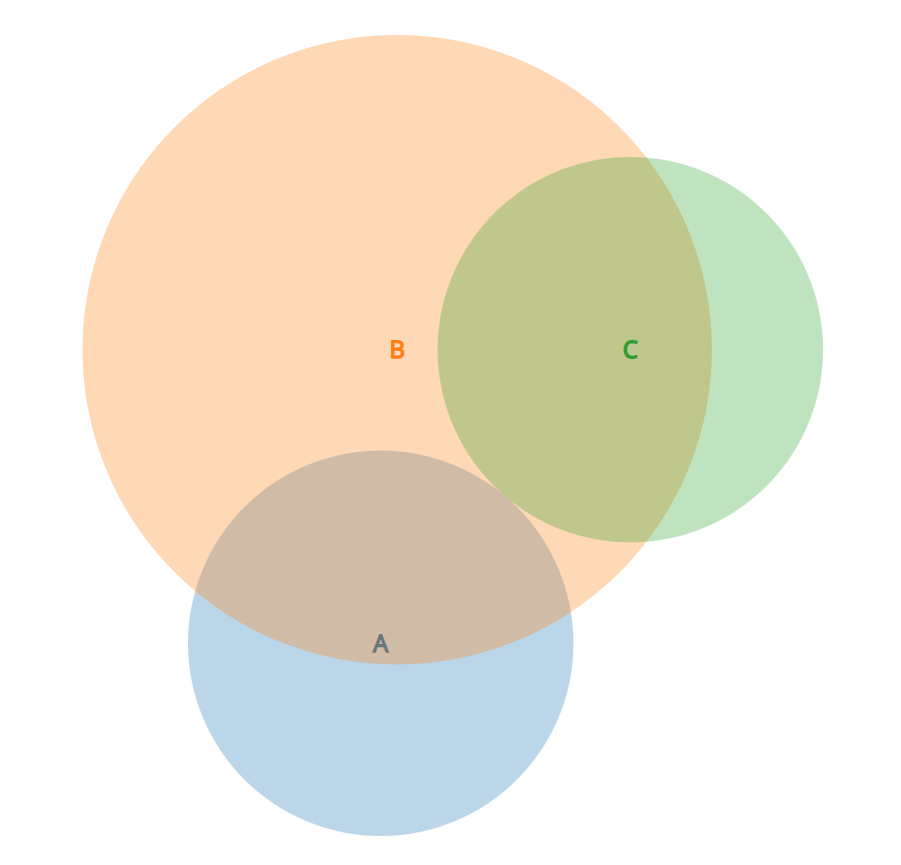
\includegraphics[width=0.3\linewidth]{Picture Folder//HW02/6-1-15-c.png}
                            \caption{6.1.15-c}
                            \label{fig:6.1.15-c}
                        \end{figure}
                    \end{enumerate}

                \item[18.] Answer questions below
                    \begin{enumerate}[a.]
                        \item Is the number $0$ in $\varnothing$? Why?
                        \item[Ans.] By definition of the empty set, it should not contain any elements. $0$ would be an element. \\
                        \item is $\varnothing = \{ \varnothing\}$? Why?
                        \item[Ans.] No, the right hand side is a set with one element, which is the empty set. But the left hand side is the empty set that contains no elements.\\
                        \item is $\varnothing \in \{\varnothing\}$? Why?
                        \item[Ans.] Yes, the empty set is an element of the set that has one element that is the empty set. \\
                        \item Is $\varnothing \in \varnothing$? Why?
                        \item[Ans.] No, $\varnothing \notin \varnothing$, since the definition of the empty set states that it should not contain any elements. If $\varnothing \in \varnothing$, that means there are an element in $\varnothing$ that is $\varnothing$ itself. 
                    \end{enumerate}
            
        \end{enumerate}

    \newpage
    \item Section 6.1 \#25, 27
        \begin{enumerate}
            \item[25.] Let  \( \ R_i = \left\{ x \in \mathbb{R} : 1 \leq x \leq 1 + \frac{1}{i} \right\} = \left[1, 1 + \frac{1}{i}\right] \ \text{for each positive integer} \ i.\), answer the following
                \begin{enumerate}[a.]
                    \item 
                    \[
                    \union{i=1}{4}R)i = \sqbkt{1,2}
                    \]
                    \item 
                    \[
                    \inter{i=1}{4}R_i = \sqbkt{1,1+\frac{1}{4}}
                    \]
                    \item They are not mutually disjoint, since
                    \[
                    \inter{i=1}{\infty}R_i = \{ 1\} \neq \varnothing
                    \]
                    \item 
                    \[
                    \union{i=1}{n}R_i = \sqbkt{1,2}
                    \]
                    \item
                    \[
                    \inter{i=1}{n}R_i = \sqbkt{1,1+\frac{1}{n}}
                    \]
                    \item
                    \[
                    \union{i=1}{\infty}R_i = \closeopen{1,\infty}
                    \]
                    \item
                    \[
                    \inter{i=1}{\infty}R_i = \{ 1\}
                    \]

                \end{enumerate}


            \item[27.] Answer questions below
                \begin{enumerate}[a.]
                    \item No, the element $d$ is in 2 different set. 
                    \item Yes,the union of every subsets are the entire set.
                    \item No, the element $4$ appeared twice.
                    \item No, the element $6$ is missing.
                    \item Yes, each element from the set $\{1,2,\ldots,9\}$ appears exactly once in the subsets, and the union of every subsets are the entire set. 
                \end{enumerate}
            
        \end{enumerate}
    \newpage

    \item Section 6.1 \#32, 33
        \begin{enumerate}
            \item[32.]  Answer the following questions
                \begin{enumerate}[a.]
                    \item Suppose $A = \{1\}$ and $B = \{u,v\}$, find $P(A \times B)$
                    \[
                    A \times B = \{ \paren{1,u},\paren{1,v}\}
                    \]
                    Now we find the power set 
                    \[
                    P\paren{A \times B} = \{\varnothing, \paren{1,u}, \paren{1,v}, \{ \paren{1,u},\paren{1,v}\}\}
                    \]

                    \item Suppose $X \in \{a,b\}$ and $Y = \{x,y\}$. Find $P(X \times Y)$
                    \[
                    X \times Y = \{ ax,ay,bx,by \}
                    \]
                    And it has the power set
                    \begin{align*}
                    P(X \times Y) =& \textcolor{blue}{\{ } \varnothing, (a, x), (a, y), (b, x), (b, y), \{(a, x), (a, y)\}, \{(a, x), (b, x)\}, \\
                    & \{(a, x), (b, y)\}, \{(a, y), (b, x)\}, \{(a, y), (b, y)\}, \\
                    &\{(b, x), (b, y)\}, \{(a, x), (a, y), (b, x)\}, \\
                    & \{(a, y), (b, x), (b, y)\}, \{(a, x), (b, x), (b, y)\}, \{(a, x), (a, y), (b, y)\}, \\
                    & \{(a, x), (a, y), (b, x), (b, y)\} \textcolor{blue}{\}}
                    \end{align*}
                \end{enumerate}

            \item[33.] Answer the following questions
                \begin{enumerate}[a.]
                    \item 
                    \[
                    P(\varnothing) = \{ \varnothing \}
                    \]
                    \item
                    \[
                    P\paren{P\paren{\varnothing}} = \{ \varnothing, \{ \varnothing \} \}
                    \]
                    \item 
                    \[
                    P\paren{P\paren{P\paren{\varnothing}}} = 
                    \{ \varnothing, \{\varnothing\} , \{\{ \varnothing \}\}, \{ \varnothing, \{ \varnothing \}\}\}
                    \]
                \end{enumerate}
        \end{enumerate}
    \newpage
    
    \item Write the following union of intervals as a single interval.
        \[
        \union{n=2}{\infty} \sqbkt{\sqrt{1 + \frac{1}{n}},\sqrt{2 - \frac{1}{n}}}
        \]
        The interval would be
        \[
        \closeopen{\sqrt{1+\frac{1}{2}}, \sqrt{2}}
        \]
    \newpage
    
    \item Section 6.2 \#6, 11, 15
        \begin{enumerate}
            \item[6.] Fill in the blanks, now for the first part
                \begin{enumerate}[(a)]
                    \item $\paren{A \cap B}\cup \paren{A \cap C}$
                    \item $x \in A$
                    \item $x \in C$
                    \item $ x \in \paren{A \cap B}\cup \paren{A \cap C}$
                \end{enumerate}
                for the second part
                \begin{enumerate}[(a)]
                    \item $vee$
                    \item $\wedge$
                    \item $ x \in A \cap \paren{B \cup C}$
                    \item set equality
                \end{enumerate}
        \end{enumerate}

        \item[11.] Prove that for all sets $A,B,C$
            \[
            A \cap \paren{B - C}\subseteq \paren{A \cap B }- \paren{A \cap C}
            \]
            \begin{proof}
                let $A,B,C$ be any set. Suppose that $x \in A$, and $x \in A \cap \paren{B-C}$. By Set Difference law, we have $B - C = B \cap C^c$, and we can rewrite the expression as
                    \[
                    x\in A \cap B \cap C^c
                    \]
                And since $x \in A$, and $A \cap B \cap C^c$, by definition of intersection we have $ x \in A \wedge x \in B \wedge x \in C^c$. Since $x \in A \wedge x \in B$, by definition of intersection we have 
                \[
                x\in A \cap B
                \]
                Also since $x \in C^c $ is equivalent to $x \notin C $, we have $x \in A \wedge x \notin C$. By definition of intersection, we have $x \notin A \cap C$, which is equivalent to $ x \in \paren{A \cap C}^c$. Since $x \in A \wedge x \in B$, and $ x \in \paren{A \cap C}^c$, by definition of intersection, we have 
                \[
                x \in \paren{A \cap B }\cap \paren{A \cap C}^c
                \]
                by law of set difference, we can therefore get
                \[
                x \in \paren{A \cap B } - \paren{A \cap C}
                \]
                since $x \in x \in A \cap \paren{B-C}$ and $x \in \paren{A \cap B } - \paren{A \cap C}$, we conclude
                \[
                A \cap \paren{B - C}\subseteq \paren{A \cap B }- \paren{A \cap C}
                \]
            \end{proof}

        \item[15.] For every set $A$, $A \cup \varnothing = A$
            \begin{proof}
                Let A be any set. Suppose that $x \in A \cup \varnothing.$ By definition of union, we have $x \in A \vee x \in \varnothing$. But $x \in \varnothing \equiv \bot$ since it contradicts the definition of empty set, therefore $x \in A$ by elimination. Since  $x \in A$ and $x \in A \cup \varnothing$, we conclude that 
                \[
                A \cup \varnothing \subseteq A
                \]
                Now we suppose $x \in A$. We get $x \in A \vee x \in \varnothing$ by generalization. Since $x \in A \vee x \in \varnothing$, by definition of intersection we get $x \in A \cup \varnothing$. Also since $x \in A$, we have obtained 
                \[
                A \subseteq A \cup \varnothing
                \]
                And by set equality
                \[
                A \cup \varnothing = A
                \]
            \end{proof}
    \newpage

    \item Section 6.2 \#22, 35
        \begin{enumerate}
            \item[22.] Prove that for all sets $A,B,C$
                \[
                A \times \paren{B \cap C} = \paren{A \times B} \cap \paren{A \times C}
                \]
                \begin{proof}
                    Suppose $(x,y) \in U$ and $x \in A \times \paren{ B \cap C}$. By definition of the Cartesian product, we have $x \in A$ and $y \in B \cap C$. Since $y \in B \cap C$, we have $y \in B$ by specialization. since $y \in B$, and $x \in A$, by definition of the Cartesian product, we have.
                    \[
                    (x,y) \in A \times B
                    \]
                    Similarly, we have $y \in C$ by specialization. And since $x \in A$ and $y \in C$, by definition of Cartesian product, we have $\paren{x,y} \in A\times C$. And since we have $\paren{x,y} \in A\times C$ and $\paren{x,y} \in A\times B$, we have 
                    \[
                    (x,y) \in \paren{A \times B} \cap \paren{A \times C}
                    \]
                    By definition of intersection. Also since $x \in A \times \paren{B \cap C} $ and $ x \in \paren{A \times B} \cap \paren{A \times C}$, we have
                    \[
                    A \times \paren{B \cap C} \subseteq \paren{A \times B} \cup \paren{A \times C}
                    \]
                    Now we suppose $(x,y) \in \paren{A \times B} \cap \paren{A \times C}$, by definition of union, we have $(x,y) \in A \times B$ and $(x,y) \in A \times C$. We have $\paren{x,y} \in A \times B$ from specialization, then $x \in A$ and $y \in B$ by definition of Cartesian product. Similarly we have $x \in A$ and $y \in C$. Since we have $y \in B $ and $y \in C$, by definition of intersection, we have $y \in B \cap C$. Since $x \in A$ and $y \in B \cap C$, by definition of Cartesian product, we have
                    \[
                    (x,y) \in A \times \paren{B \cap C}
                    \]
                    Also since $(x,y) \in \paren{A \times B} \cap \paren{A \times C}$, we have
                    \[
                    \paren{A \times B} \cap \paren{A \times C} \subseteq  A \times \paren{B \cap C}
                    \]
                    And we have 
                    \[
                    A \times \paren{B \cap C} = \paren{A \times B} \cap \paren{A \times C}
                    \]
                    by definition of set equality. 
                \end{proof}

                \item[35.] Prove that for all sets $A,B,C$, if $A \subseteq B$ and $B \cap C =\varnothing$, then $A \cap C = \varnothing$.
                    \begin{proof}
                        Suppose $A,B,C$ are any set, suppose $A \subseteq B$, and $B \cap C = \varnothing$. Let $x \in U$ and $x \in A$. By definition of subset, since $A \subseteq B$, then $x \in A \then X \in B$. Since $x \in A$, then we have $x \in B$. Since $B \cap C = \varnothing$, $B^c \cup C^c = U$, by DeMorgan's Law and Complement of empty set. We know $x \in U$, therefore $ x \in B^c$ or $x \in C^c$. We know $ x \in B$, which means $ x\notin B^c$, then by specialization, we have $x \in C^c$, which means $x \notin C$. We now know if $x \in A$ then $x \notin C$, by definition of intersection, $A \cap C = \varnothing$.
                    \end{proof}
                
        \end{enumerate}

        
        




\end{enumerate}


\section{draft}
\subsection{5.4-Q6}
For a polygon to be convex means that given any two points on or inside the polygon, the line joining the points lies entirely inside the polygon. Use mathematical induction to prove that for every integer \( n \geq 3 \), the interior angles of any \( n \)-sided convex polygon add up to \( 180(n - 2) \) degrees.

\textbf{Proof (by mathematical induction):} Let \( P(n) \) be the following statement:

The interior angles of any \( n \)-sided convex polygon add up to \( 180(n - 2) \) degrees.

\textbf{Base Case:} 

Show that \( P(3) \) is true: \( P(3) \) is the statement that the interior angles of any 3-sided convex polygon add up to \( 180 \times (3 - 2) \) degrees.

\( P(3) \) is true because any 3-sided polygon is a triangle, and the interior angles of such a polygon add up to 180 degrees, which equals \( 180 \times (3 - 2) \) degrees.

\textbf{Inductive Step:} 

Show that for each integer \( k \geq 3 \), if \( P(k) \) is true, then \( P(k + 1) \) is true: Let \( k \) be any integer with \( k \geq 3 \), and suppose that \( P(k) \) is true. In other words, suppose that the interior angles of any \( k \)-sided convex polygon add up to \( 180(k - 2) \) degrees. [This is \( P(k) \), the inductive hypothesis.]

We must show that \( P(k + 1) \) is true. Complete the proof and submit it as a free response.

\newpage

\subsection{2}

Suppose that \( f_0, f_1, f_2, \ldots \) is a sequence defined as follows:
\[
f_0 = 5, \quad f_1 = 16, 
\]
\[
f_k = 7f_{k-1} - 10f_{k-2} \quad \text{for every integer } k \geq 2.
\]

Prove that \( f_n = 3 \cdot 2^n + 2 \cdot 5^n \) for each integer \( n \geq 0 \).

\textbf{Proof by strong mathematical induction:} Let the property \( P(n) \) be the equation \( f_n = 3 \cdot 2^n + 2 \cdot 5^n \). 

We will show that \( P(n) \) is true for every integer \( n \geq 0 \).

\textbf{Base Cases:} 

Show that \( P(0) \) and \( P(1) \) are true:

For \( P(0) \):
\[
f_0 = 3 \cdot 2^0 + 2 \cdot 5^0 = 3 \cdot 1 + 2 \cdot 1 = 5
\]

For \( P(1) \):
\[
f_1 = 3 \cdot 2^1 + 2 \cdot 5^1 = 3 \cdot 2 + 2 \cdot 5 = 6 + 10 = 16
\]

Thus, \( P(0) \) and \( P(1) \) are true because \( 3 \cdot 2^0 + 2 \cdot 5^0 = 5 \) and \( 3 \cdot 2^1 + 2 \cdot 5^1 = 16 \).

\textbf{Inductive Step:} 

Show that for every integer \( k \geq 1 \), if \( P(i) \) is true for each integer \( i \) from 0 through \( k \), then \( P(k + 1) \) is true:

Let \( k \) be any integer with \( k \geq 1 \), and suppose that for every integer \( i \) with \( 0 \leq i \leq k \), \( f_i = 3 \cdot 2^i + 2 \cdot 5^i \). This is the \textbf{inductive hypothesis}. We must show that \( f_{k + 1} = 3 \cdot 2^{k+1} + 2 \cdot 5^{k+1} \).

Now, by the definition of \( f_0, f_1, f_2, \ldots \),
\[
f_{k + 1} = 7f_k - 10f_{k-1}.
\]

Using the inductive hypothesis, we substitute the expressions for \( f_k \) and \( f_{k-1} \):
\[
f_k = 3 \cdot 2^k + 2 \cdot 5^k, \quad f_{k-1} = 3 \cdot 2^{k-1} + 2 \cdot 5^{k-1}.
\]

Thus,
\[
f_{k + 1} = 7(3 \cdot 2^k + 2 \cdot 5^k) - 10(3 \cdot 2^{k-1} + 2 \cdot 5^{k-1}).
\]

Expanding and simplifying,
\[
f_{k + 1} = 21 \cdot 2^k + 14 \cdot 5^k - 30 \cdot 2^{k-1} - 20 \cdot 5^{k-1}.
\]

\[
= 21 \cdot 2^k - 30 \cdot 2^{k-1} + 14 \cdot 5^k - 20 \cdot 5^{k-1}.
\]

\[
= 3 \cdot 2^{k+1} + 2 \cdot 5^{k+1}.
\]

Thus, \( f_{k + 1} = 3 \cdot 2^{k+1} + 2 \cdot 5^{k+1} \).

This completes the proof by induction.


\newpage

\subsection{3}
\textbf{Proof by Mathematical Induction:}

We will prove the following statement by induction:

For all nonnegative integers \( n \),
\begin{itemize}
    \item If \( n \) is even, the units digit of \( 9^n \) is 1.
    \item If \( n \) is odd, the units digit of \( 9^n \) is 9.
\end{itemize}

\textbf{Base Case:}

For \( n = 0 \) (even), we have \( 9^0 = 1 \). The units digit is 1.

For \( n = 1 \) (odd), we have \( 9^1 = 9 \). The units digit is 9.

Thus, the statement holds for the base cases.

\textbf{Inductive Step:}

Assume that the statement holds for some nonnegative integer \( k \), that is:

\begin{itemize}
    \item If \( k \) is even, the units digit of \( 9^k \) is 1.
    \item If \( k \) is odd, the units digit of \( 9^k \) is 9.
\end{itemize}

We need to prove the statement holds for \( k+1 \).

\textbf{Case 1:} \( k \) is even.

If \( k \) is even, then the units digit of \( 9^k \) is 1. We need to show that the units digit of \( 9^{k+1} \) is 9.

\[
9^{k+1} = 9 \cdot 9^k
\]

The units digit of \( 9^k \) is 1, so the units digit of \( 9 \cdot 9^k \) is the same as the units digit of \( 9 \cdot 1 = 9 \). Hence, the units digit of \( 9^{k+1} \) is 9.

\textbf{Case 2:} \( k \) is odd.

If \( k \) is odd, then the units digit of \( 9^k \) is 9. We need to show that the units digit of \( 9^{k+1} \) is 1.

\[
9^{k+1} = 9 \cdot 9^k
\]

The units digit of \( 9^k \) is 9, so the units digit of \( 9 \cdot 9^k \) is the same as the units digit of \( 9 \cdot 9 = 81 \). Thus, the units digit of \( 9^{k+1} \) is 1.

\textbf{Conclusion:}

By the principle of mathematical induction, the statement holds for all nonnegative integers \( n \). That is, if \( n \) is even, the units digit of \( 9^n \) is 1, and if \( n \) is odd, the units digit of \( 9^n \) is 9.

\[
\subsetneq
\]













\end{document}